\chapter{The Fundamentals of Mode-Matching}\label{fund_mm}
	  The plane wave and the spherical wave represent the two extremes of transverse spatial confinement. The former is a collimated beam that has one steady wavefront whose normal vector is parallel with the axis of propagation, whereas the latter type of wave has a single point of origin and its normal rays diverge in all directions.  There exists a solution which is a medium between the two cases called a Gaussian beam.  When dealing with length sensing degrees of freedoms such as section \ref{FP}, the simple plane wave approximation is sufficient in describing the dynamics, however, when trying to understand the misalignment and mode-mismatch signals, it is necessary to incorporate Gaussian beams and associated their higher order modes.
		\section{Gaussian Beam Optics}
		Consider the famous Maxwell's equations:
		\begin{equation}
		\label{18.1:1}
		\begin{aligned}
		 \nabla \times \mathbf{E} &=-\frac{\partial \mathbf{B}} {\partial t}
		\\\nabla \cdot \mathbf{B} &=0				
		\\\nabla \times \mathbf{B} &= \mu\ \mathbf{J} + \frac{1}{c^2} \frac{\partial \mathbf{E}} {\partial t}
		\\
		\nabla \cdot \mathbf{E} &= \frac{\rho}{\epsilon}
		\end{aligned}
		\end{equation}
		
		Concentrating on the electric field in vacuum, we arrive at the Helmholtz Equation
		\begin{equation}\label{Helmholtz}
		(\nabla^2 + k^2 ) \mathbf{U}(\mathbf{r},t) = 0
		\end{equation}
		
		where $k=\frac{2\pi\nu}{c}$ is the wave number and $\mathbf{U}(\mathbf{r},t)$ is the complex amplitude which can describe either the electric or magnetic fields.  There are a variety of solutions to equation \ref{Helmholtz} which include the plane and spherical waves \cite{Saleh}.  These two types of solutions are the extremes when considering the angle and spatial distribution as a function of propagation.  The plane wave which has been used in chapter \ref{intro} is a beam whose rays have no variance in the spatial direction as it propagates through space, whereas the spherical wave starts at a point and spreads as a function of distance from the origin. Somewhere in between these two extrema is the paraxial wave which is a wave pattern that has its rays at small angles relative to the direction of propagation (see Figure[raysoflight]).  It is possible to express the paraxial solution to equation \ref{Helmholtz} as a plane wave with a modulated complex envelope $\mathbf{A}(r)$
		\begin{equation}
		\mathbf{U}(\mathbf{r}) = \mathbf{A}(\mathbf{r}) e^{-ikz}
		\end{equation}
		However, in order for the paraxial wave to exist, $\mathbf{U}(r)$ must satisfy the Helmholtz equation or alternatively, the complex amplitude portion must satisfy a separate differential equation known as the paraxial Helmholtz Equation. By imposing the constraints which force the envelope to vary slowly with respect to the z-axis within the distance of one wavelength $\lambda = 2\pi/k$,

		\begin{subequations}
		\begin{equation}\label{paraxiala}
		\bigg| { \frac{\partial^2 \mathbf{A}}{\partial z^2} } \bigg|  \ll  \bigg| { k {\frac{\partial\mathbf{A}}{{\partial z}} } } \bigg|
		\end{equation}
		\begin{equation}\label{paraxialb}
		\bigg| { \frac{\partial^2 \mathbf{A}}{\partial z^2} } \bigg|  \ll  \bigg| { k {\frac{\partial^2 \mathbf{A}}{\partial x^2}} } \bigg|
		\end{equation}
		\begin{equation}\label{paraxialc}
		\bigg| { \frac{\partial^2 \mathbf{A}}{\partial z^2} } \bigg|  \ll  \bigg| { k{\frac{\partial^2 \mathbf{A}}{\partial y^2}}} \bigg|
		\end{equation}
		\end{subequations}
		
		the partial differential equation which arises is called the Paraxial Helmholtz Equation:
		
		\begin{equation}\label{paraHelmholtz}
		\nabla_T^2 A(r) - i2k \frac{\partial A(r)}{\partial z} = 0
		\end{equation}
		
		where $\nabla_T^2 = \frac{\partial^2}{\partial x^2} + \frac{\partial^2}{\partial y^2} $ is the transverse Laplacian.  A simple solution for equation \ref{paraHelmholtz} is the complex paraboloidal wave
		
		\begin{equation} \label{complexenvelope}
		A(\mathbf{r}) = \frac{A_0}{q(z)} e^{\frac{-ikr^2}{2q(z)}} , \quad q(z)=z+iz_0
		\end{equation}
		
		where $z_0$ is the Rayleigh range and is directly proportional to the square of the waist size.  In order to separate the amplitude and phase portions of the wave, it is useful to rewrite $q(z)$ as
		
		\begin{equation}\label{invq}
		\frac{1}{q(z)} = \frac{1}{R(z)} - i \frac{\lambda}{\pi W^2(z)}
		\end{equation} 
		
		Plugging equation \ref{invq} into \ref{complexenvelope} leads directly to the complex amplitude for a Gaussian Beam
		\begin{equation}
		U(r,z) = A_0 \frac{W_0}{W(z)} e^{-\frac{r^2}{W^2(z)}} e^{-ikz - ik \frac{r^2}{2R(z)} + i \phi(z)}
		\end{equation}
		where
		\begin{subequations}
		\begin{equation}
		W(z) = W_0 \sqrt{1 + \bigg( \frac{z}{z_0} \bigg)^2}
		\end{equation}
		\begin{equation}\label{ROC}
		R(z) = z \bigg[ 1 + \bigg( \frac{z}{z_0} \bigg)^2 \bigg]
		\end{equation}
		\begin{equation}\label{gouy}
		\phi(z)= \text{tan}^{-1}\bigg(\frac{z_0}{z}\bigg)
		\end{equation}
		\begin{equation}
		W_0 = \sqrt{\frac{\lambda z_0}{\pi}}
		\end{equation}
		\end{subequations}
	
		The Gaussian beams are named as such because of the intensity distribution,
		\begin{equation}
		I(r,z) = \vert U(r,z) |^2 = I_0 \bigg[ \frac{w_0}{w(z)}\bigg]^2 \exp \bigg[ \frac{-2 r^2}{w^2(z)}\bigg]
		\end{equation}
		where $I_0 = \vert A_0\vert^2$ and has a peak at $r=0$ and $z=0$.  The width increases as the beam propagates along the $\hat{z}$ axis away from the waist position and the intensity maximum on the beam axis decreases (see Figure \ref{fig:GaussIntensity}),
		\begin{equation}
		I(0,z) = \frac{I_0}{1 + (z/z_0)^2}
		\end{equation}
		When it comes to sensing a laser beam, the most common way is using a photodetector which is a transducer that transforms the integrated intensity or power into an electronic current.  
		
		\begin{figure}[ht]
			\centering
			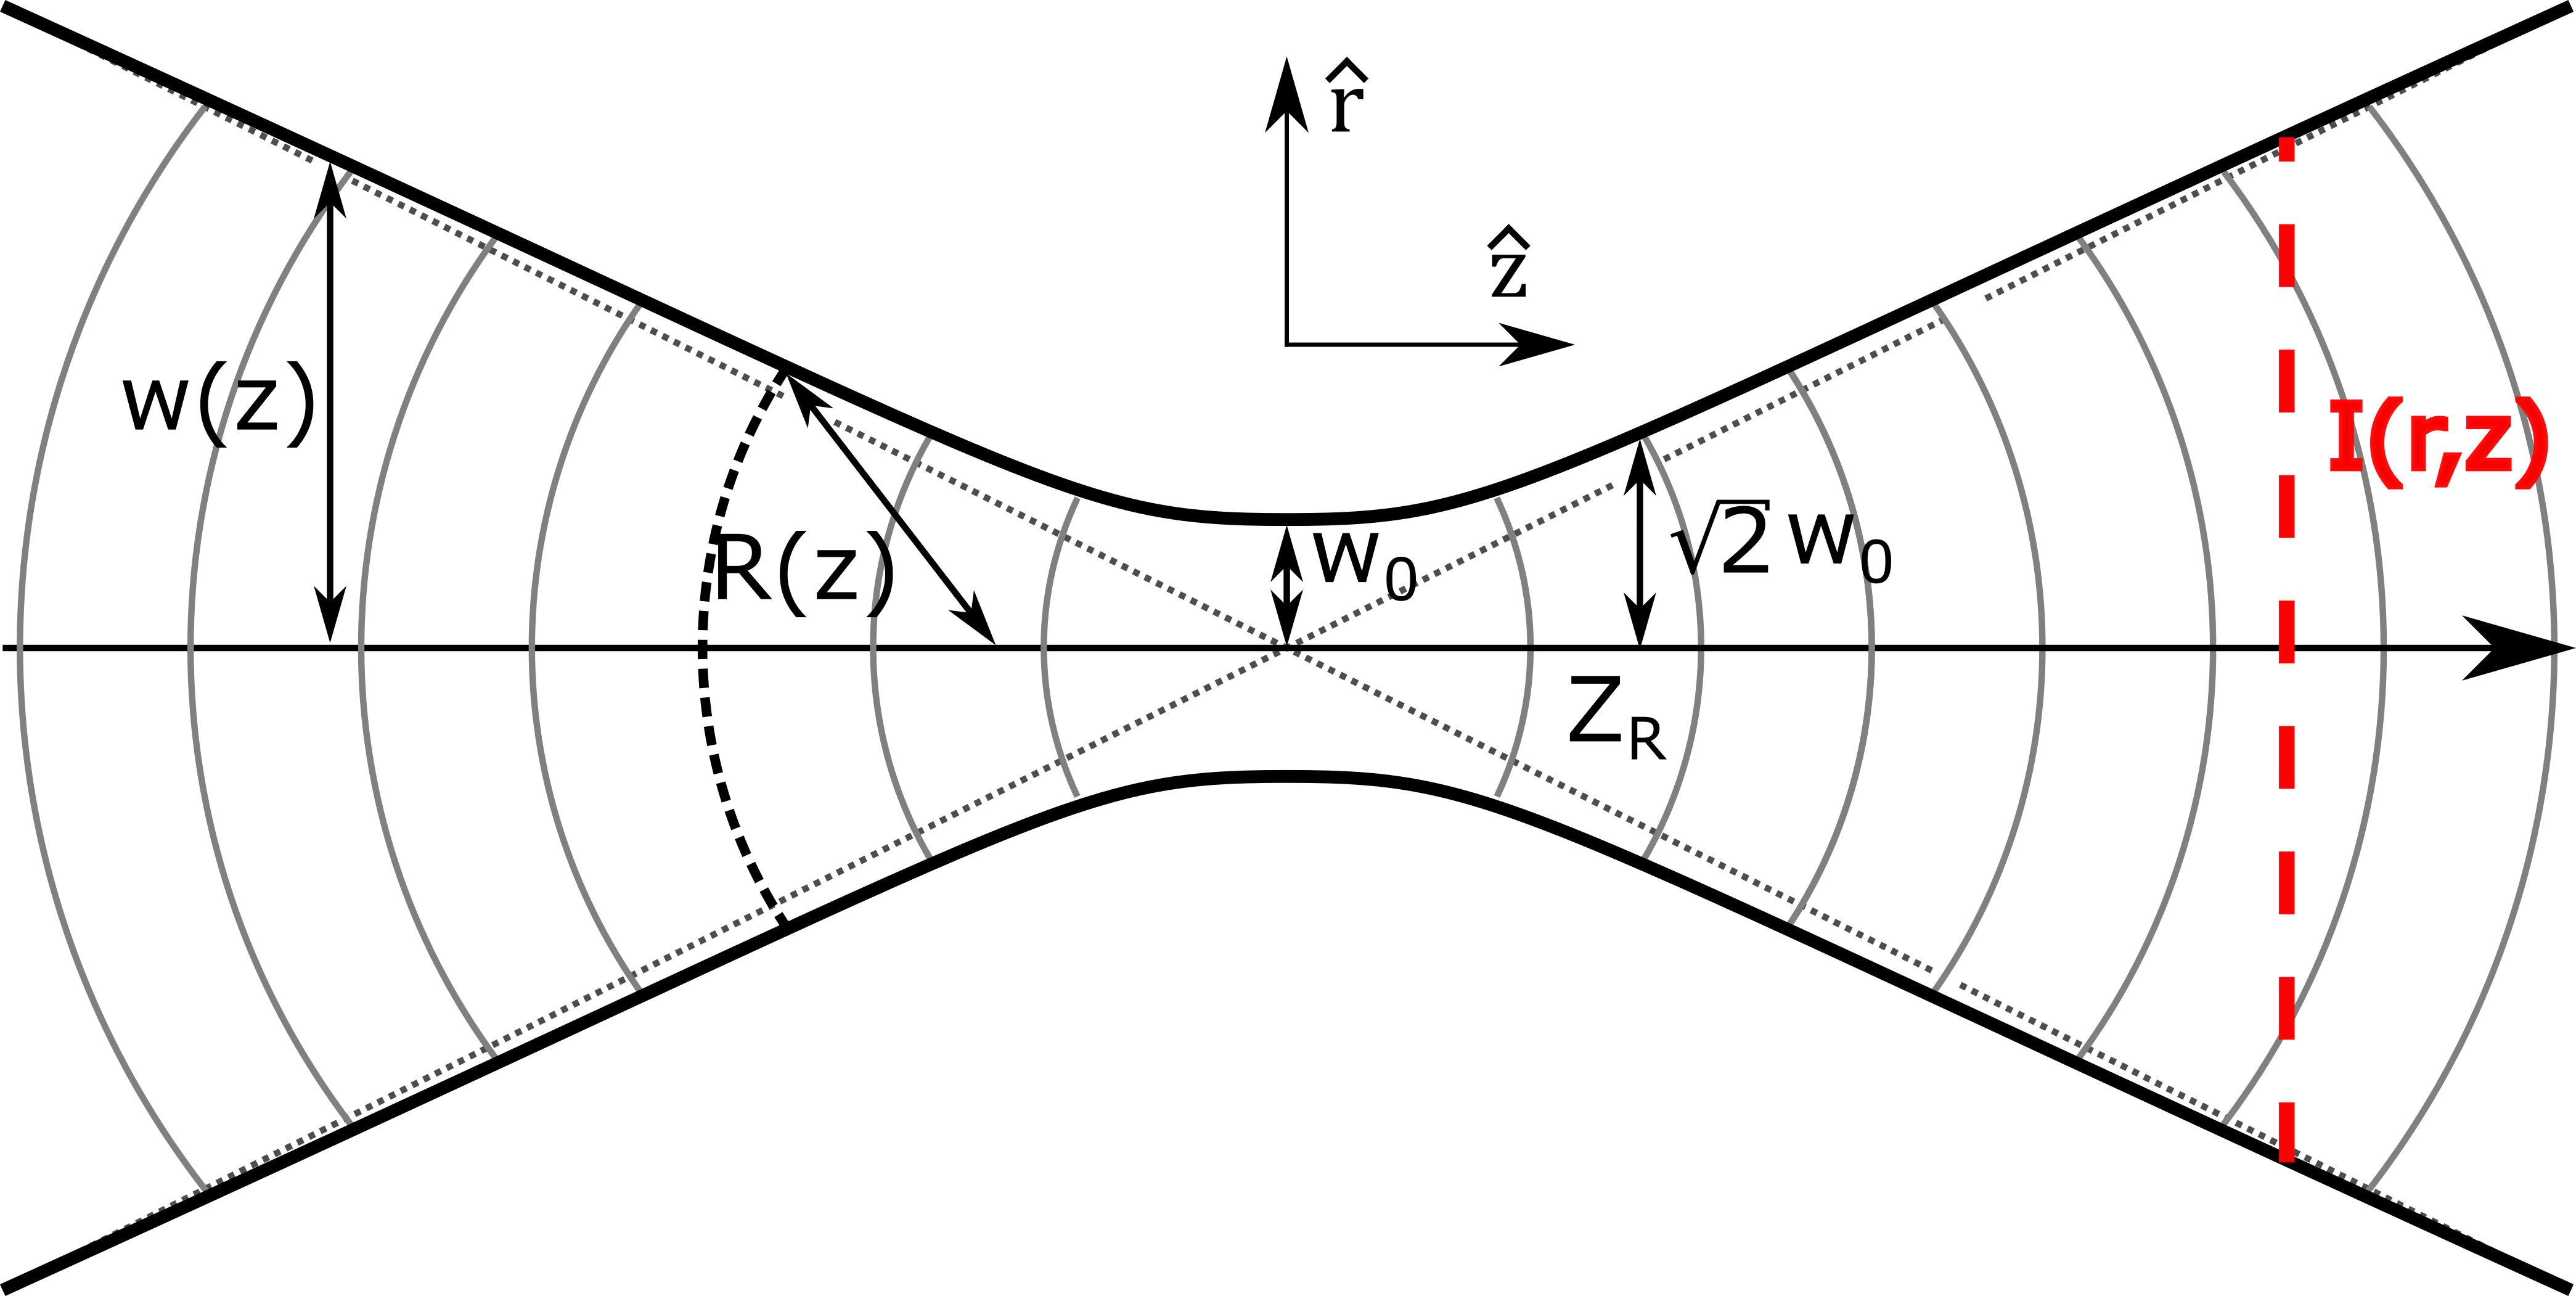
\includegraphics[width=0.65 \textwidth]{../Figures/GaussProfile.png}
			\caption[A depiction of the Gaussian beam properties with respect to cylindrical coordinates.]
			{\textbf{A depiction of the Gaussian beam properties with respect to cylindrical coordinates.} Because the beam is axially symmetric, the two coordinates are denoted by $\hat{r}$ for the radial and $\hat{z}$ for the axis of propagation with the origin located at the center. The thick dark lines represent the beam size, $w(z)$, which is minimal at the waist, $w(z)=w_0$ when $z=0$ and asymptotic towards $\lambda/\pi w_0$ when $z \approx \inf$ as shown by the dotted gray lines. The red dashed line represents the intensity cross section of the beam which changes to a wider and flatter profile as a function of distance from the waist.}
			\label{fig:GaussProfile}
		\end{figure}
	
		\begin{figure}[ht]
			\centering
			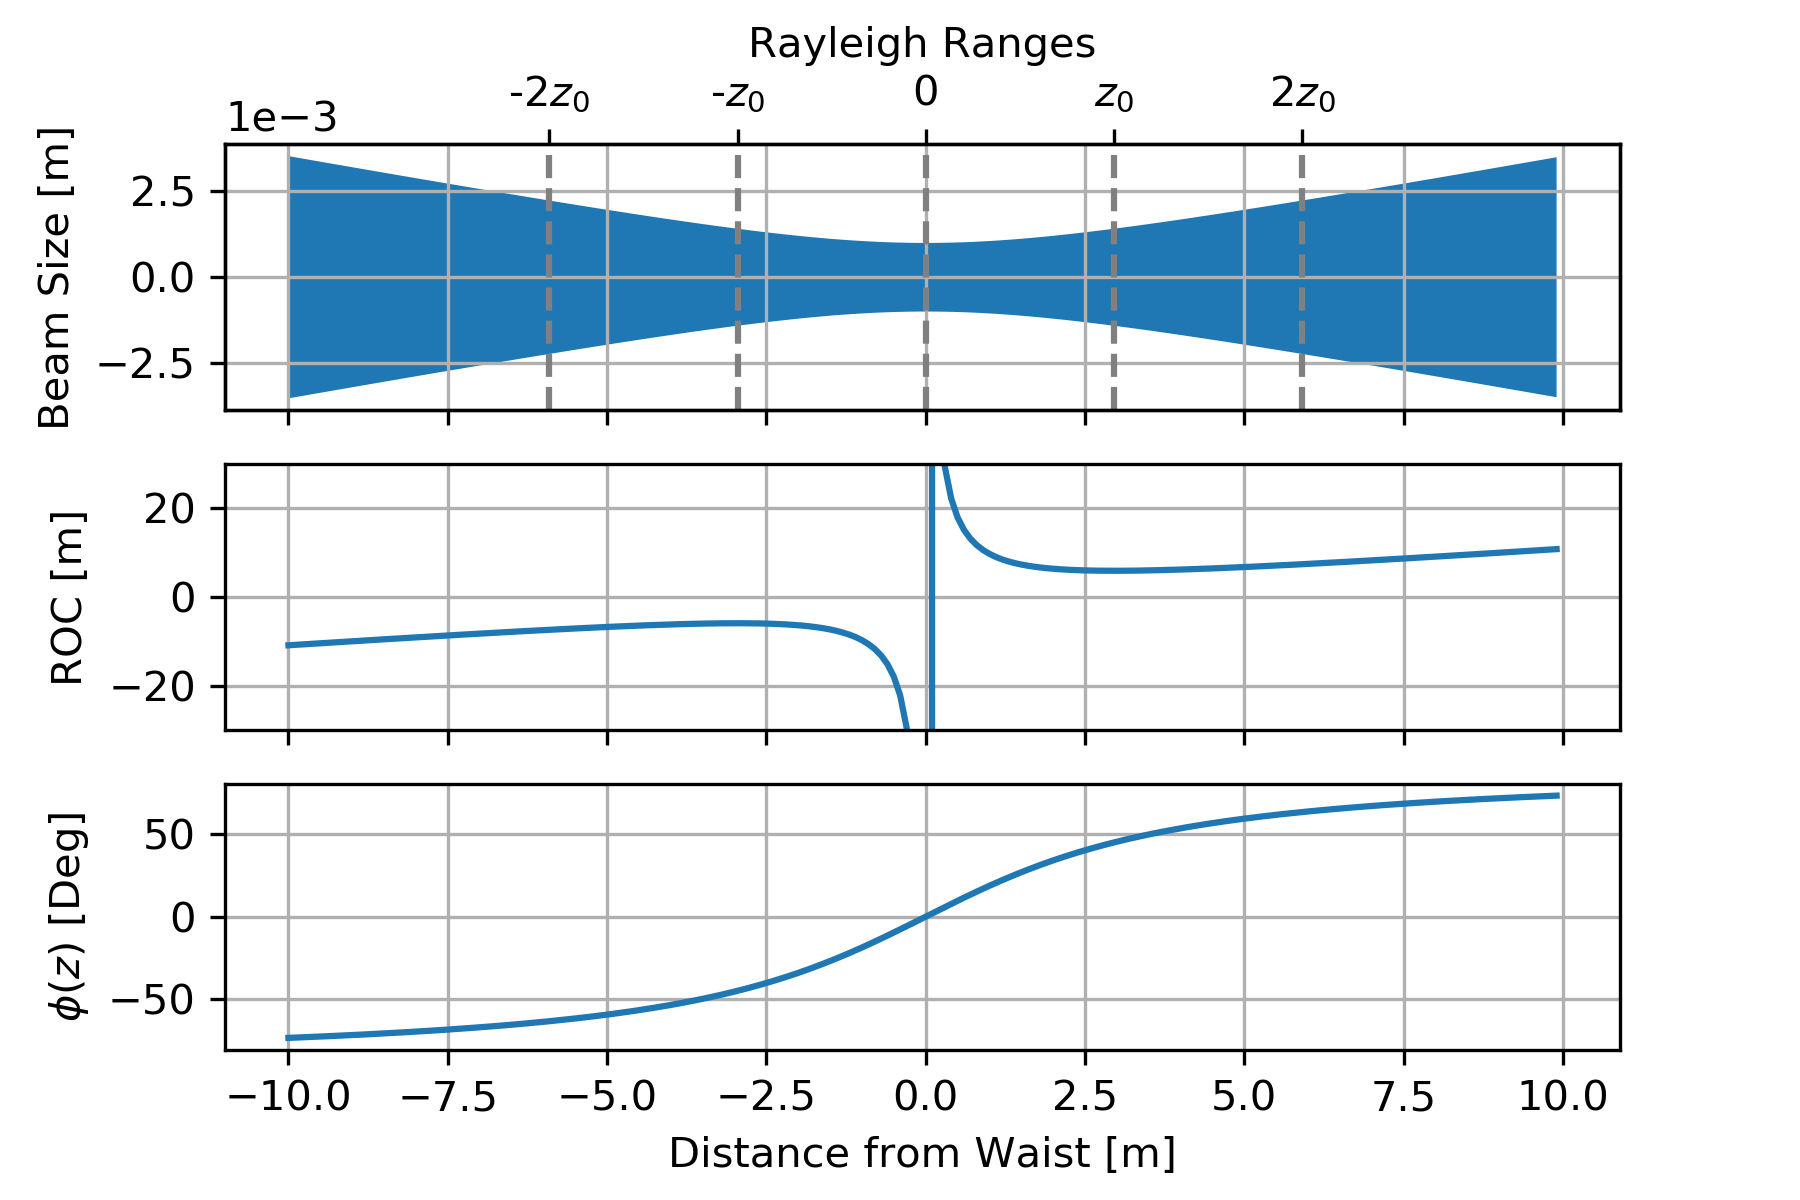
\includegraphics[width=0.85 \textwidth]{../Figures/GaussBeamParams.png}
			\caption[Beam size, radius of curvature, and Gouy phase as a function of distance propagation from the waist.] 
			{\textbf{Beam size, radius of curvature, and Gouy phase as a function of distance propagation from the waist.} The vertical dashed gray lines represent the integer number of Rayleigh ranges.  At the point $z=z_0$, the beam size is $\sqrt{2}$ of the waist size and the radius of curvature is minimal.  At this point, the Gouy phase propagation is lagging the plane wave by $\pi /4$ and the beam intensity is half of that at the waist.}
			\label{fig:GaussParams}
		\end{figure}

		\begin{figure}[ht]
			\centering
			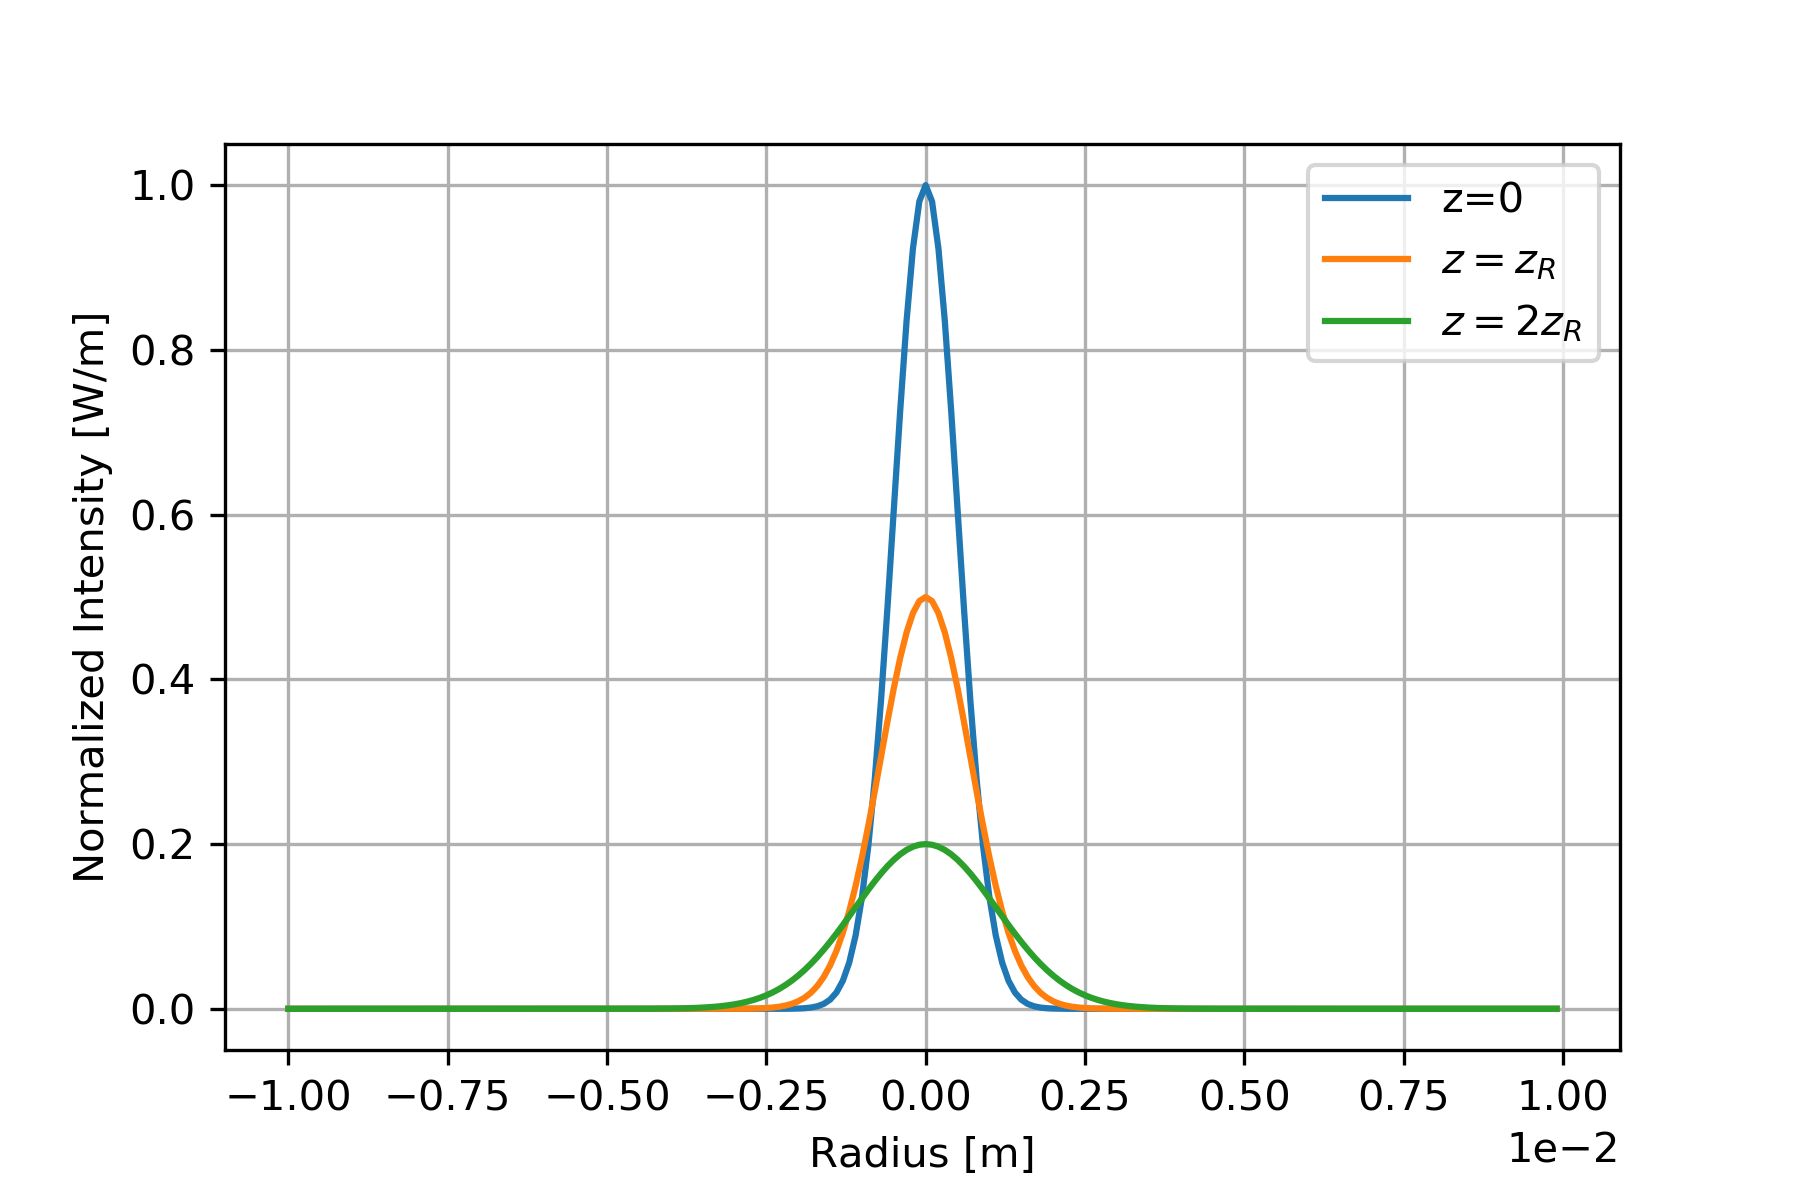
\includegraphics[width=0.65 \textwidth]{../Figures/GaussBeamIntensity.png}
			\caption{Intensity}
			\label{fig:GaussIntensity}
		\end{figure}

		\subsubsection{Gouy Phase}
		The Gouy phase given by equation \ref{gouy} is the phase lag between a Gaussian beam and a perfect plane wave that occurs as a function of propagation along the $\hat{z}$-axis which ranges from $\phi(z) = \pm \pi/2$ for $z =\pm \inf$.  Physically, this could be interpreted as the difference between the laser beam behaving like a plane wave when $z\approx0$ (or near field) and eventually evolving into a spherical wave when $z\approx \pm \inf$ (or far field) (see Figure \ref{fig:GaussParams} ).  Although this phenomenon is interesting mathematically, most texts do not consider how to practically use or measure the Gouy phase.  In LIGO technical notes and electronic logs, the Gouy phase of sensors or actuators are used to describe where along the beam path the piece of equipment is located.  This will indicate what degree of freedom is being observed or adjusted.  For example, in ray optics \cite{Saleh} a laser beam has two degrees of freedom, the displacement and angle from the optical axis.  If an actuator such as a piezo-electric transducer with an attached reflective mirror is placed near the origin or focus of the laser beam, then the controlled degree of freedom is only the angle.  Alternatively, if the actuator is placed in the far field then the controlled degree of freedom is almost entirely displacement.  This is also true of sensors at various points along the $\hat{z}$-axis to determine the exact alignment of the optical beam.
		
		In practice, it is impossible to sense the true waist of an optical system because it could be inside a Fabry-Perot cavity.  So the clever designer must insert a pick-off beam to sample the transmission or reflection of the interested optical system and use a combination of lenses to create a telescope for the sensors and infers the degrees of freedom.  Then, by rotating to the two-dimensional space created by the sensors to represent the interested space spanned by the optical system's degrees of freedom; colloquially, this is known as a sensing matrix.  Using this method, sensors do not have to be exactly at the near or far field because it is only required that the two sensors are separated by $\pi/2$ in Gouy phase, in fact, it is usually easier to place one sensor at $+\pi/4$ and the other at $-\pi/4$. 
		
		Unfortunately, there is no transducer that directly measures the Gouy phase so in order to \textit{determine} the Gouy phase of a particular sensor or actuator, one must model the beam propagation and fit the waist location.
		
		\subsubsection{Hermite-Gauss Modes}
		The fundamental Gaussian beam is not the only solution which can be used to solve equation \ref{paraHelmholtz}.  In fact, there exists a complete set of solutions that can solve the paraxial Helmholtz Equation in rectangular coordinates, which are referred to as the Hermite Gauss modes
		\begin{equation}\label{HG}
		\begin{aligned}
		&U_{mn}(x,y,z) = A_{mn}\bigg[ \frac{W_0}{W(z)} \bigg] \mathbb{G}_m\Bigg( \frac{\sqrt{2}x}{W(z)}  \Bigg) \mathbb{G}_n\Bigg( \frac{\sqrt{2}y}{W(z)} \Bigg)\\
		&\times \text{exp} \bigg\{ -ikz - \frac{ik(x^2+y^2)}{2R(z)} + i(m+n+1)\phi(z) \bigg\}
		\end{aligned}
		\end{equation}
		
		where,
		\begin{equation}
		\mathbb{G}(u) = \mathbb{H}(u) \, \text{exp}(-u^2/2)
		\end{equation}
		
		and $ \mathbb{H}(u)$ are the well known Hermite polynomials.  It is important to mention that the Gouy phase of the complex amplitude is different than the fundamental Gaussian beam by a factor of $(m + n + 1)$ and that the intensity distribution of these higher order modes are much different. Both of these facts will become extremely important in the following wavefront sensing discussion.
		
		The extra Gouy phase that a higher order mode accrues as a function of $z$ shows up as in the frequency or cavity length domain as one sweeps through a full free spectral range using an offset in the length or frequency error signal.  This  can be directly used to measure the higher order mode separation and becomes important if the cavity has a low finesse which means the fundamental Gaussian mode has a spread comparable in frequency to the first order mode then it is easy to hop from one to the other.
		\begin{figure}[ht]
			\centering
			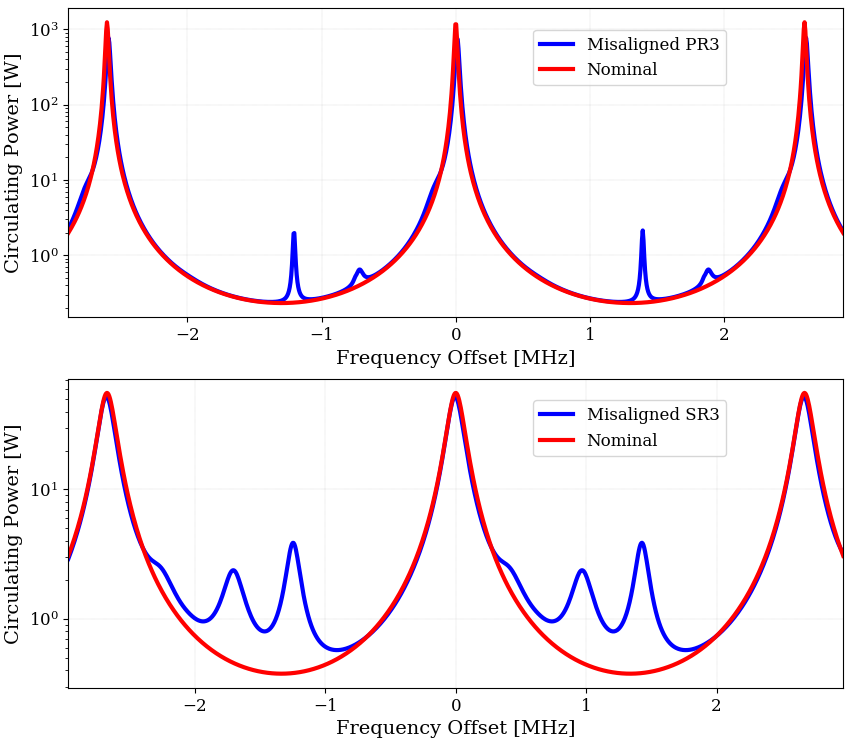
\includegraphics[width=0.65 \textwidth]{../Figures/PRC_SRC_ModeScan.png}
			\caption[A Finesse model of a longitudinal mode scan comparing the Advanced LIGO power recycling and signal recycling cavities.]
			{\textbf{A Finesse model of a longitudinal mode scan comparing the Advanced LIGO power recycling and signal recycling cavities}	The upper and lower plots is represent of the PRC and SRC, respectively.  The main difference between these two optical cavities is obvious when comparing the three large peaks corresponding to the 00 mode resonances.  The power recycling cavity has a much higher and sharper peak which indicates higher finesse where as the signal recycling cavity is a much lower finesse which has a broader and shorter peak.  The red traces are with nominal alignment where as the blue lines correspond to misalignments of PR3 and SR3 by $1 \mu$rad which allow higher order mode content to resonant as a function of length.}
			\label{fig:PRC_SRC_mode_scan}
		\end{figure}
	
	
		\subsubsection{Laguerre Modes}
		Another complete set of alternative solutions to equation \ref{paraHelmholtz} exists which are called the Laguerre-Gauss modes
		
		\begin{equation}\label{LG}
		\begin{aligned}
		&V_{\mu\nu}(\rho,\theta,z) = A_{\mu\nu}\bigg[ \frac{W_0}{W(z)} \bigg] \mathbb{L}^{\mu}_{\nu} \Bigg( \frac{\sqrt{2}x}{W(z)}  \Bigg) \\
		&\times \text{exp} \bigg\{-ikz-\frac{ik\rho^2}{2R(z)} + i(\mu+2\nu+1)\phi(z) \bigg\}
		\end{aligned}
		\end{equation}
		
		where $\mathbb{L}^{\mu}_{\nu} \Bigg( \frac{\sqrt{2}x}{W(z)}  \Bigg)$ is the Laguerre polynomial function. Both equations \ref{HG} and \ref{LG} are able to fully describe any complex electromagnetic amplitude; and because they both form complete sets, there is a rotation which can map from one basis to the other \cite{BEIJERSBERGEN} \cite{ONeilModeTransform}
		
		\begin{equation}
		U^{LG}_{\mu \nu} (x,y,z) = \sum\limits_{k}^{N} i^k b(n,m,k) U^{HG}_{N-k,k} (x,y,z)
		\end{equation}
		where
		\begin{equation}
		b(n,m,k) = \sqrt{\bigg( \frac{(N-k)!k!}{2^N n!m!} \bigg)} \frac{1}{k!} \frac{\text{d}^k}{\text{d}t^k}[(1-t)^m (1+t)^m]\vert_{t=0}
		\end{equation}

		\subsection{Misalignment and Higher Order Modes}\label{Misalign}
		Morrison and Anderson \cite{Anderson} \cite{Morrison} derived a simplistic way of how small misalignments and mode mismatch in cavities can couple the fundamental Gaussian beam into various higher order modes.  This is done by taking a linear cavity and using its perfectly matched Gaussian beam as a reference, and then varying the input electric field with small perturbations and expanding in terms of the higher order modes.  So long as the mismatches are small, it is possible to consider only the first few terms of the expansion which have gained most of their power from the fundamental mode.
		
		Consider the first three Hermite-Gauss modes of equation \ref{HG} in one dimension and normalized to set the total optical power to unity:

		\begin{equation}
		\label{Gauss1D}
		\begin{aligned}
				U_{0}(r) & =	\bigg( \frac{2}{\pi w^2(z)} \bigg)^{1/4}  e^{-r^2/w^2(z)}		&
		\\		U_{1}(r) &	=	\bigg( \frac{2}{\pi w^2(z)} \bigg)^{1/4}  \frac{2r}{w(z)} \quad e^{-r^2/w^2(z)}&,
		\\	 	U_{2}(r) &	=	\bigg( \frac{2}{\pi w^2(z)} \bigg)^{1/4}  \frac{1}{\sqrt{2}} \bigg( \frac{4r^2}{w^2(z)} - 1 \bigg)   e^{-r^2/w^2(z)}
		\end{aligned}
		\end{equation}
				
		\subsubsection{Beam Axis Tilted}
		If the input beam into an optical cavity is tilted by an angle $\alpha$ with respect to the nominal cavity axis, the wave front of the input beam will have an extra phase propagation relative to the cavity that is approximately proportional to $e^{ik \alpha r}$.  By implementing the small angle approximation, which is valid if the misalignment is much smaller than the divergence angle of the fundamental mode $k \alpha r << 1$, the resultant input beam is
		
		\begin{equation}
		\Psi \approx U_{0}(r) e^{ik \alpha r} \approx U_{0}(r) ( 1 + ik \alpha r ) =  U_{0}(r) + \frac{ik \alpha w(z)}{\sqrt{2\pi}} U_{1}(r)
		\end{equation}
		
		Here the factor associated with the first higher order mode is complex, indicating there is a 90 degree phase difference between the fundamental and off axis mode. 
		\subsubsection{Beam Axis Displaced}
		If the input beam is displaced in the transverse direction by a quantity $\Delta r$, the resultant waveform will be
		
		\begin{equation}
		\begin{aligned}
			\Psi 	&=  		U_{0}(r + \Delta r	) 
			\\		&= 			\bigg( \frac{2}{\pi w^2(z)} \bigg)^{1/4}  e^{-(r+\Delta r)^2/w^2(z)}
			\\		&= 			\bigg( \frac{2}{\pi w^2(z)} \bigg)^{1/4}  e^{-(r^2 + 2r \Delta r  + \Delta r^2)/w^2(z)}
			\\		&\approx 	\bigg( \frac{2}{\pi w^2(z)} \bigg)^{1/4}  e^{-r^2/w^2(z)} e^{-2r \Delta r/w^2(z)}
			\\		&\approx 	\bigg( \frac{2}{\pi w^2(z)} \bigg)^{1/4}  e^{-r^2/w^2(z)} \bigg(1 - \frac{2r \Delta r}{w^2(z)} \bigg)
			\\		&=			\bigg( U_0(r) - \sqrt{\frac{2}{\pi}} \frac{\Delta r }{w(z)} U_1(r)	 \bigg)
		\end{aligned}
		\end{equation} 
		
		Similarly to a tilted input beam axis, the displaced beam axis couples power to the first higher order mode, however, the latter does not have a 90 degree phase difference previously seen in the former.  This point is of extreme importance when trying to discern between the two effects as shown in Section [].  Although comparing the two cases in Figure, one can already seen the difference between the wavefronts in the near field, $z<<z_R$, and the far field, $z>>z_R$.  
		
		In the near field, there is no phase difference due to a displaced beam, but there is one for a tilted beam.  Conversely, in the far field, there is no phase difference due to a tilted beam, but there is one from a displaced beam.  In order to implement a closed loop feedback system, the wavefront sensors discussed in Section \ref{WFS} will use this precise logic to extract an error signal.
		
		\subsection{Mode Mismatch and Higher Order Modes}\label{Modemismatch}
		
		\subsubsection{Waist Size Shifted}
		By considering the effect of evaluating the fundamental mode at the waist position, $z=0$, but changing the waist size by a small amount $\epsilon$, it is possible to see coupling into higher order modes by expanding to first order.	
		\begin{equation}
		\begin{aligned}
		\Psi 	&=  		U_{0} \big(r,w(z) = w_0/(1+\epsilon) \big) 
		\\		&= 			\bigg( \frac{2}{\pi w_0^2} \bigg)^{1/4} \sqrt{1 + \epsilon} \quad e^{-r^2 (1+\epsilon)^2/w_0^2 }
		\\		&\approx 	\bigg( \frac{2}{\pi w_0^2} \bigg)^{1/4} (1 + \epsilon /2) \quad e^{-r^2/w_0^2} \quad e^{-2r^2\epsilon/w_0^2} 
		\\		&\approx 	\bigg( \frac{2}{\pi w_0^2} \bigg)^{1/4} (1 + \epsilon /2) \quad e^{-r^2/w_0^2} \quad (1-2r^2\epsilon/w_0^2)
		\\		&\approx 	\bigg( \frac{2}{\pi w_0^2} \bigg)^{1/4} \bigg(1+ 2\epsilon\bigg(\frac{1}{4} - \frac{r^2}{w_0^2}\bigg) \bigg ) \quad e^{-r^2/w_0^2}	
		\\		&=			U_0(r) \, - \, \frac{\epsilon}{\sqrt{2}} \, U_2(r)
		\end{aligned}
		\end{equation}
		Changing the waist size by a small amount will couple the fundamental mode to the in-phase second order Hermite Gauss mode.
		
		\subsubsection{Waist Position Shifted}
		To repeat the process from above with a waist position shift, it is useful to start with a more general equation that includes the phase that is gained from including the radius of curvature,
		
		\begin{equation}\label{EFieldwPhase}
		\Psi = 	\bigg( \frac{2}{\pi w^2(z)} \bigg)^{1/4} \quad e^{-r^2/w^2(z)} \quad e^{-ikr^2/2R(z)}
		\end{equation}
		where $R(z)$ is from equation \ref{ROC}.  It is also useful to approximate the shift in waist position along the longitudinal axis is small compared to the Rayleigh range of the beam, $\Delta z << z_0$, which leaves the waist size approximately the same and the radius of curvature inversely proportional to the shift. 
		
		\begin{subequations}
		\begin{align}
		\begin{split}
			w^2(\Delta z)	&= 	w^2_0 \bigg[1 + \bigg(\frac{\Delta z}{z_0}  \bigg)^2 \bigg]  \approx	w^2_0
		\end{split}\\
		\begin{split}
			R(\Delta z) 	&=	\Delta z \bigg(1 + \bigg(\frac{z_0}{\Delta z}\bigg)^2\bigg) \approx	\frac{z_0^2}{\Delta z}
		\end{split}
		\end{align}
		\end{subequations}

		Plugging the equations above into \ref{EFieldwPhase},
		
		\begin{equation}
		\begin{aligned}
		\Psi 	&\approx	\bigg( \frac{2}{\pi w_0^2} \bigg)^{1/4} \quad e^{-r^2/w_0^2} \quad e^{-ikr^2 \Delta z /2 z_0^2}
		\\		&\approx	\bigg( \frac{2}{\pi w_0^2} \bigg)^{1/4} \quad e^{-r^2/w_0^2} \quad \bigg( 1-\frac{ikr^2 \Delta z}{2 z_0^2}  \bigg)
		\\		&=			U_0(r) - \bigg( \frac{2}{\pi w_0^2} \bigg)^{1/4} e^{-r^2/w_0^2} \quad \frac{ikr^2 \Delta z}{2 z_0^2}
		\\		&=			U_0(r) - i \frac{\Delta z}{2k w_0^2} \bigg( 4U_2(r) + U_0(r) \bigg)
		\end{aligned}
		\end{equation}
		
		The equations above show that a fundamental Gaussian mode that is shifted in waist position will couple power to the second order Hermite Gauss mode.  Although changes in the waist size or position couple power to the same mode, they differ by a 90 degrees in phase as denoted by the extra factor of $i$ in the coupling coefficient.  By recognizing the two effects are in different quadrature phases will allow a user to design a system to distinguish between the different types of physical couplings, this is shown in Section \ref{WFS}.
		
		 In order to be physically valid one would need to consider the full two dimensional space so that the equation would encapsulate the full transverse mode, however, the x and y components would follow the exact same derivation. On that point, it is important to note that only the mode mismatch couplings from either a varying waist position or size has higher order modes that are circularly symmetric.
		
		\section{Wavefront Sensing}\label{WFS}
		Heterodyne detection via modal decomposition of the full electric field allows the use of wavefront sensors to extract an error signal from the optical system.  Hefetz et.al \cite{HefetzWFS} created a formalism to describe the use of wavefront sensors by creating frequency sidebands which accumulate a different Gouy phase than the electric field at the carrier frequency when passed through the optical system.  By observing the demodulated signal of the intensity, it is possible to obtain a linear signal that corresponds to a physical misalignment or mode mismatch.
		
		Fundamentally, the purpose of wavefront sensing is to detect the content of higher order modes due to physical disturbances of the optical cavity (ie. mode mismatch or misalignment).  In other words, it is examining the difference between the incoming beam's and the cavity's eigenmodes.
		
		Consider a general equation for an electric field which is a linear combination of all higher order modes of the complex amplitude
		\begin{equation}
		E(x,y,z) = \sum\limits_{m,n}^{\infty} a_{mn} U_{mn}(x,y,z)
		\end{equation}
		
		where $ U_{mn}(x,y,z)$ are the eigenmodes described in equation \ref{HG} (or \ref{LG}) and $a_{mn}$ is the complex amplitude.  It is also convenient in the following analysis to use vectors when describing the composition of the electric fields.
		
		\begin{equation}\label{EVector}
		\ket{E(x,y,z)} = \begin{pmatrix} E_{00} 
		\\ E_{01}
		\\E_{10}
		\\E_{20}
		\\E_{02}
		\end{pmatrix}
		\end{equation}

		When creating a theory that involves laser beams, it is useful to define operators that are important in describing physical situations.  For example, laser beams propagate through space and pick up phase according to equation \ref{HG} which can be represented by the spatial propagation operator,
		
		\begin{equation}
		\hat{P}_{mn,kl} = \delta_{mn} \delta_{kl} \quad \text{exp}[-ik(z_2 - z_1)] 
		\\ \text{exp}[i(m+n+1)\phi(z)]
		\end{equation}

		However, it is useful to compare how the fundamental Gaussian mode propagates compared to the higher order modes,

		\begin{equation} \label{GouyPhaseMatrix}
		\hat{\eta}_{\mu \nu} = 
		\begin{pmatrix}
		e^{i\phi}	&0			&0			& 0 			& 0
		\\ 0		&e^{2i\phi}	&0			& 0				& 0
		\\ 0		&0			&e^{2i\phi}	& 0				& 0
		\\ 0		&0			&0			& e^{3i\phi}	& 0
		\\ 0		&0			&0			& 0				& e^{3i\phi}
		\end{pmatrix}
		\end{equation}

		From the above diagonal elements, it is clear that the higher order modes have an extra phase compared to the fundamental 00 mode, this effect will be extremely important on how an error signal can be derived from the optical system.
		
		\begin{equation}
		\ket{E(x,y,z_2)} = \hat{M}(x,y,z_1,z_2)	\ket{E(x,y,z_1)}
		\end{equation}
		
		where $\hat{M}(x,y,z_1,z_2)$ is the misalignment operator.  Since we are using the paraxial approximation, the z-components of the misalignment operator are small so we can approximate $\hat{M}_(x,y,z_1,z_2) \approx \hat{M}_(x,y)$ and the expectation value is
		
		\begin{equation}
		M_{mn,kl}=  \bra{U_{mn}(x,y,z_1)} M(x,y) \ket{U_{kl}(x,y,z_2)}
		\end{equation}

		where the product is an integral over the transverse space $\int \!\!\! \int_{D(x,y)} \text{d}x \text{d}y$

		\begin{equation} \label{misalign_matrix}
		\hat{\Theta}_{\mu \nu} = 
		\begin{pmatrix}
		   1			&2i\theta_x		&2i\theta_y		& 0 & 0
		\\ 2i\theta_x	&1				&0				& 0	& 0
		\\ 2i\theta_y	&0				&1				& 0	& 0
		\\ 0			&0				&0				& 1	& 0
		\\ 0			&0				&0				& 0	& 1
		\end{pmatrix}
		\end{equation}

		\begin{equation} \label{mistrans_matrix}
		\hat{\mathbb{D}}_{\mu \nu} = 
		\begin{pmatrix}
			1					&\alpha_x/\omega_{0}	&\alpha_y/\omega_{0}	& 0 & 0
		\\ \alpha_x/\omega_{0}	&1						&0						& 0 & 0
		\\ \alpha_y/\omega_{0}	&0						&1						& 0	& 0
		\\ 0					&0						&0						& 1	& 0
		\\ 0					&0						&0						& 0 & 1 
		\end{pmatrix}
		\end{equation}
		
		\begin{equation} \label{waistloc_matrix}
		\hat{\mathbb{Z}}_{\mu \nu} = 
		\begin{pmatrix}
		1				&0		&0		&\Delta z_x 	&\Delta z_y  
		\\ 0			&1		&0		&0 				&0
		\\ 0			&0		&1		&0 				&0
		\\ \Delta z_x	&0		&0		&1 				&0
		\\ \Delta z_y	&0		&0		&0				&1 
		\end{pmatrix}
		\end{equation}
		
		where $\Delta z_{(x,y)} =  \frac{i}{\sqrt{2}} \frac{\lambda b}{2\pi\omega_{0}} $
		
		\begin{equation} \label{waistsize_matrix}
		\hat{\mathbb{Z}}_{0, \mu \nu} = 
		\begin{pmatrix}
		1					&0		&0		&\Delta z_{0,x} 	&\Delta z_{0,y} 
		\\ 0				&1		&0		&0 					&0
		\\ 0				&0		&1		&0 					&0
		\\ \Delta z_{0,x} 	&0		&0		&1 					&0
		\\ \Delta z_{0,y} 	&0		&0		&0					&1 
		\end{pmatrix}
		\end{equation}

		where $\Delta z_{0,(x,y)} =   \frac{1}{\sqrt{2}} \frac{\omega'-\omega_{0}}{\omega_{0}} $

		Figure: Beat frequency between two modes.
	
	